\documentclass[12pt,a4paper,english]{article}
\usepackage[latin1]{inputenc}
\usepackage[T1]{fontenc}
\usepackage[english]{babel}
\usepackage{graphicx}
\usepackage{fancyhdr}
\usepackage{geometry}
\usepackage{helvet}
\usepackage{epsfig}
\usepackage{textcomp} % degree celsius
\usepackage{natbib}
\usepackage{afterpage}
\usepackage{amssymb}
\usepackage{subfigure}
\usepackage{float}
\usepackage{tabularx}
\usepackage{multirow}
\usepackage[footnotesize,sl]{caption}
\usepackage{pdfpages}
\usepackage{enumerate}
\usepackage{babel}
\usepackage{lineno}
\usepackage{color, colortbl}
\usepackage{draftwatermark}
\usepackage{caption}
\usepackage{setspace}
\usepackage{amsmath}
\usepackage{array}
%\captionsetup{labelformat=empty}
\definecolor{Gray}{gray}{0.88}
\definecolor{DarkGray}{gray}{0.7}
\SetWatermarkText{DRAFT}
\SetWatermarkScale{3}
\renewcommand{\baselinestretch}{1.50}\normalsize
\newcolumntype{x}[1]{% 
>{\centering\arraybackslash\hspace{0pt}}p{#1}}%

%\geometry{verbose,a4paper,tmargin=25mm,bmargin=17mm,lmargin=17mm,rmargin=17mm}
\geometry{verbose,a4paper,tmargin=20mm,bmargin=17mm,lmargin=17mm,rmargin=17mm}

\setcounter{secnumdepth}{4} 

\begin{document}

\bibliographystyle{ams}
%\bibliographystyle{harvard}

\thispagestyle{empty}

\setpagewiselinenumbers
\modulolinenumbers[5]
\linenumbers

\vspace{8mm}

\begin{center}

\vspace{6mm}

{\LARGE Bayesian hierarchical modelling of extreme hourly precipitation in Norway}
%\title{Bayesian hierarchical modelling of extreme hourly precipitation in Norway}

\vspace{6mm}

{\large Anita Verpe Dyrrdal$^{1,2}$,.......... }
%\author{Anita Verpe Dyrrdal$^{1,2}$,.....}

%\maketitle

\vspace{6mm}

\noindent $^{1}$ The Norwegian Meteorological Institute, PO Box 43 Blindern, 0313 Oslo, Norway \\E-mail: Anita.Dyrrdal@met.no \\
$^{2}$ University of Oslo, Department of Geosciences, PO Box 1047 Blindern, 0316 Oslo, Norway\\
$^{3}$ Norwegian Computing Center, PO Box 114 Blindern, 0314 Oslo, Norway

\end{center}

\vspace{10mm}

\begin{abstract}

\noindent Abstract.....

\end{abstract}

\newpage

\section{Introduction}

Heavy rainfall over a short period of time often causes damage to infrastructure, and thus represents an economic challenge as well as a threat to human safety. Such intense events are driven by complex spatio-temporal processes and are usually characterized by limited predictability and small spatial extent, which challenges a sparse observational network. Nevertheless, in the planning and design of important infrastructure, such as road and railway and urban environment, there is a great need for spatially continuous estimates of extreme short-duration precipitation. In addition to the large spatial variability and relatively few observational sites, the complex terrain and different weather systems that hit Norway further complicates such a task. In this study we present maps of extreme hourly precipitation in Norway, created from advanced statistical tools that distribute extremal properties of available measurements in space through their relationship to more acquainted variables.

Hierarchical latent variable models (CORRECT NAME??) is one of the statistical approaches that recently have been applied in the modeling of spatial extremes, along with e.g. copulas and max-stable random fields. \cite{Davisonetal2012} performed a review of the three above-mentioned methods, applied on summer maximum daily rainfall in the Plateau region of Switzerland. They found that, although a latent variable approach is flexible, it does not give a realistic picture of the spatial structure of extreme events. However, this drawback does not affect the models capability of computing the spatial distribution of marginal properties, which is confirmed by \cite{ApputhuraiandStephenson2013}.
 
In the model applied here we introduce Bayesian inference to make use of any prior knowledge and to obtain a measure of uncertainty, which has long been a shortcoming in return level estimation in Norway. We refer to the model as a Bayesian Hierarchical Model (BHM), where the variable of interest is assumed to be conditionally independent on an unobserved latent process, and the posterior distribution is simulated through a Markov chain. \cite{Cooleyetal2007} were the first to apply this type of model for daily precipitation threshold exceedance. They estimated parameters describing the Generalized Pareto distribution, and were able to produce maps of return levels for daily precipitation in Colorado, US. 

As the first to our knowledge, we here attempt to apply a Bayesian Hierarchical Model to spatially distribute the parameters of a Generalized Extreme Value (GEV) distribution for hourly precipitation in Norway, with the aim of producing maps of extremes. We believe this is currently among the best alternatives to create spatially continuous high-resolution maps, including a measure of uncertainty. The maps can easily be updated with increased time series lengths and future observational sites. 

\section{Extreme value theory}

Extreme precipitation is often referred to in terms of return levels, which is a measure of the frequency of rainfall events of a certain intensity and duration. To estimate return levels we need to know the distribution of the extremes. Extreme value theory states that block maxima of any variable follow a GEV distribution described by the three parameters location ($\mu$), scale ($\sigma$) and shape ($\xi$) \citep{Coles2001}, in the following way

\begin{equation}
G(x) = exp\{ - [1 + \xi(\frac{z - \mu}{\sigma})]^{-\frac{1}{\xi}}\}  
\end{equation}

\noindent The distribution can be any of three types, depending on the value of $\xi$; Weibull ($\xi<0$), Fr\'echet ($\xi>0$), and Gumbel ($\xi=0$). Rainfall is, according to literature, assumed to follow a Fr\'echet distribution, characterized by a fat tail and no convergence \citep{Wilks1993, KoutsoyiannisandBaloutsos2000, Katzetal2002, Colesetal2003, ColesandPericchi2003, Koutsoyiannis2004a}. The Fr\'echet distribution also represents the lowest risk for engineering structures.

The return level $z_p$ associated with the return period $frac{1}{p}$, can be obtained from

\begin{equation}
z_p = \Bigg\{ \begin{array}{lr} \mu - \frac{\sigma}{\xi}[1 - \{ - log(1 - p)\}^\xi], & \xi \neq 0\\
\mu - \sigma log\{ - log(1 - p)\}, & \xi = 0
\end{array}
\end{equation}

\noindent $z_p$ is expected to be exceeded on average once every $frac{1}{p}$ years, or in any particular year with probability p.

\section{Hourly precipitation measurements}

Two types of rain gauges are used to measure hourly precipitation in Norway; Tipping bucket and weight pluviometer. In Norway the first tipping bucket stations were established in the spring of 1967 and the first weight pluviometer stations in December 1991. The quality of the tipping bucket measurements are quite good, while some weight pluviometer stations are associated with technical difficulties resulting in erroneous values. Data used in the current study have undergone a ``cleaning-process'' (ref. Mamen...), deleting unrealistic values and obvious errors. In the further analysis, we ended up using annual maxima from 59 tipping bucket stations and 10 weight pluviometer stations. Time series lengths vary from 10 to 45 years.

In addition to the network of stations being sparse, the spatial distribution is highly inhomogeneous. As seen in Fig.~\ref{data:fig1}, the majority of stations are located in the south, and especially in the surroundings of Oslo. The latter is, however, not all negative as the southern parts usually experience the most intense and local showers, requiring a denser network. A lack of observations obviously introduces great uncertainty and represents a challenge when attempting to distribute the statistical characteristics in space.

\begin{figure}[htbp]
\begin{center}
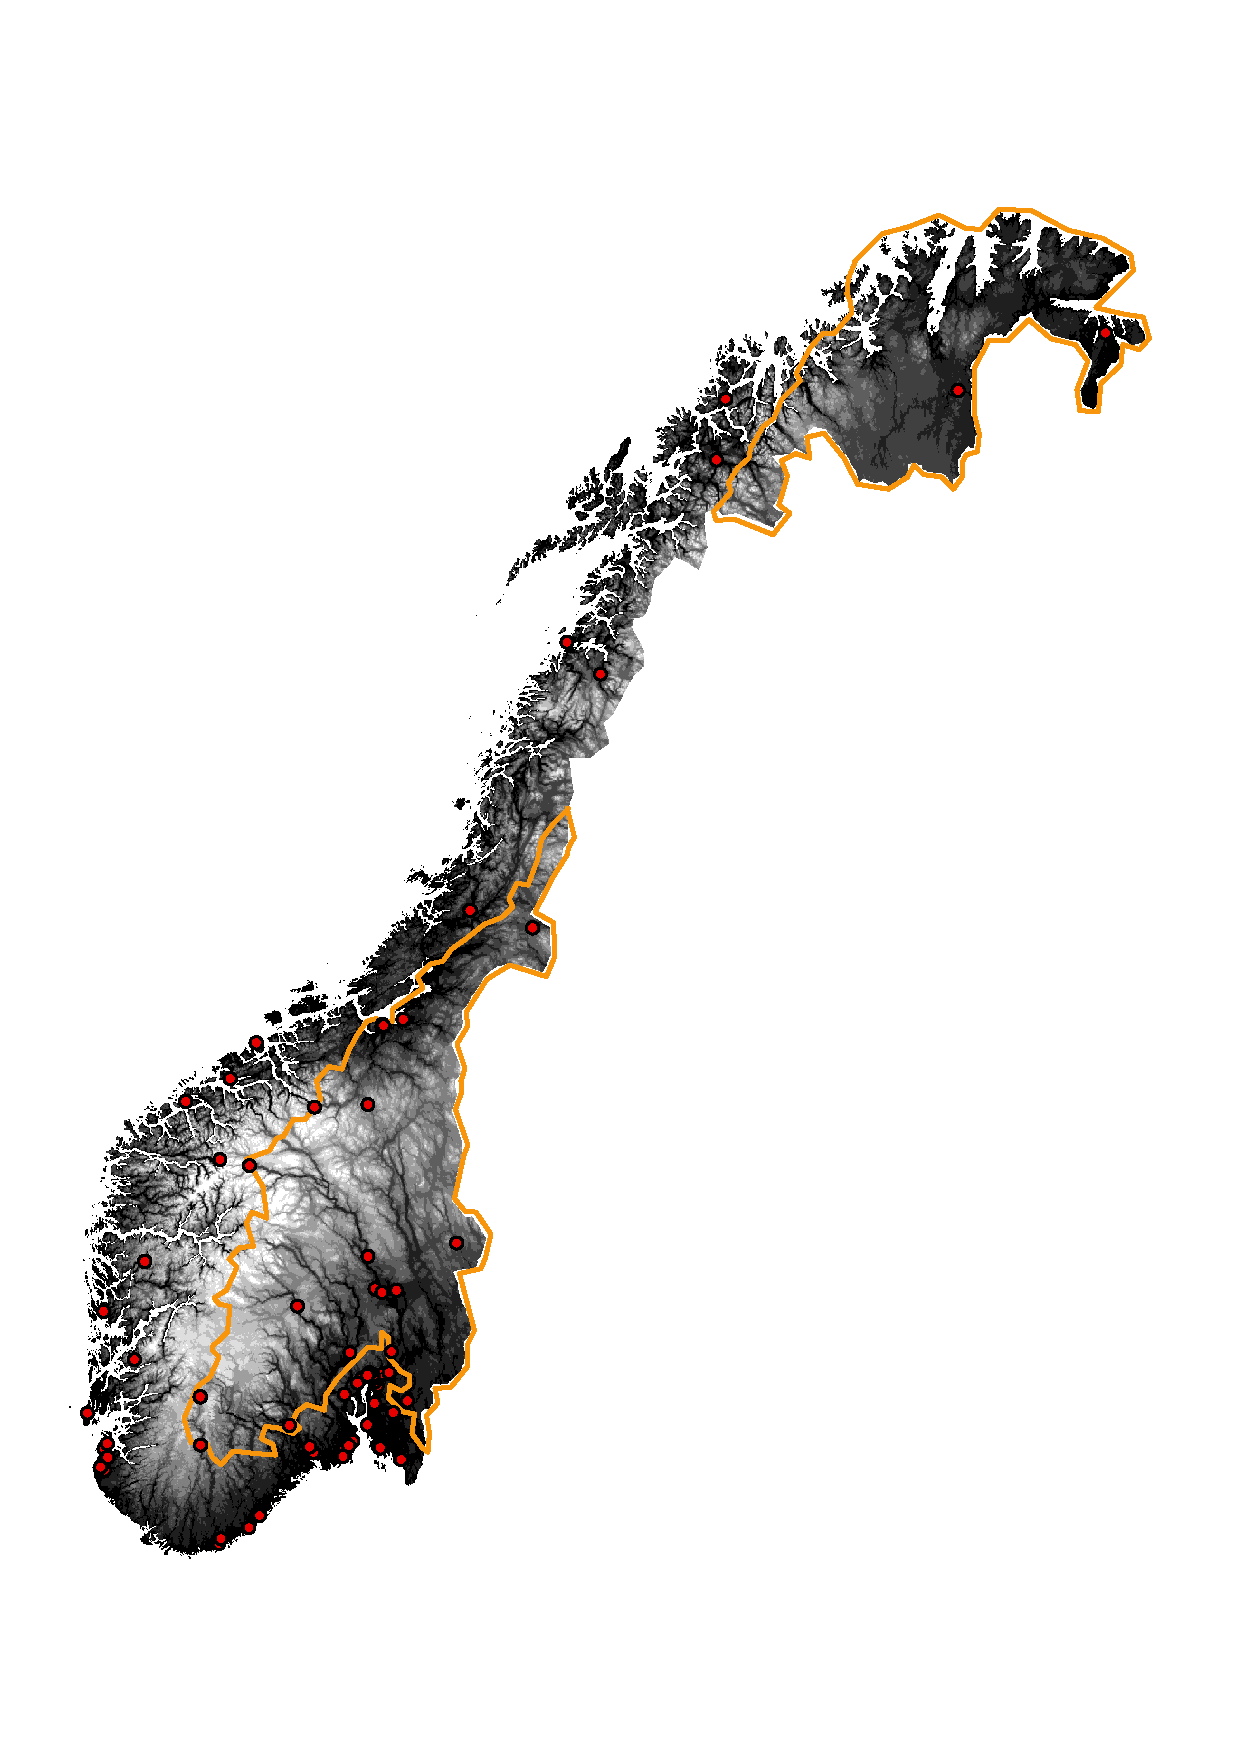
\includegraphics[width = 0.5\linewidth]{Figs/stations.pdf} 
\end{center}
\caption[stations]{\label{data:fig1}Map of Norway with stations (red dots) and area dominated by summer precipitation (orange line). The topography is shown in black and white.}
\end{figure}

\section{Bayesian Hierarchical Model (BHM) for spatial extremes}

The R-package SpatialExtremes version 2.0-0 (http://spatialextremes.r-forge.r-project.org/) provides several tools for the modeling of spatial extremes. Here we apply the package to generate a Markov chain from a BHM for annual maximum hourly rainfall, assuming they are GEV distributed and conditionally independent. The GEV parameters, $\mu$, $\sigma$, and $\xi$, are also assumed to vary smoothly in space according to a stochastic process, and each parameter is characterized by mutually independent Gaussian processes. Thus, the parameters can be described as follows:

\begin{equation}
y(x) = f_{y(x)}(x;\beta_{y}) + S_{y}(x;\alpha_{y},\lambda_{y},\kappa_{y}),
\end{equation}

\noindent where $f_{y}$ is a deterministic function depending on the regression parameters $\beta_{y}$, and $S_{y}$ is a stationary Gaussian process with zero mean and a covariance function with hyperparameters sill ($\alpha_{y}$), range ($\lambda_{y}$), and smooth ($\kappa_{y}$). $\alpha_{y}$, $\lambda_{y}$ and $\kappa_{y}$ describe the spatial dependence in the GEV parameters. The powered exponential covariance model was chosen to describe the Gaussian latent process.

The spatial distribution of the GEV parameter can be modeled through a hierarchical setup composed by three layers: 1. Data layer, 2. Process layer, and 3. Prior layer. 
	
\begin{enumerate}
\item In the data layer, a GEV distribution is fitted to annual maximum hourly precipitation from point measurements, using maximum likelihood estimation (MLE) to approximate the GEV parameters.

\item The process layer introduces explanatory variables or covariates (here) that link the GEV parameters to more familiar geographical and climatological characteristics, thus describing the latent process. We tested 11 different covariates, presented in section 2.3, and several combinations of these. All covariates and coordinates were standardized to have a mean of zero and a standard deviation of one before included in the model.

\item In the prior layer, Bayesian priors are assigned to the hyperparameters characterizing the latent process. An inverse gamma is used for $\alpha_{y}$, while a gamma prior is assumed for $\lambda_{y}$ and $\kappa_{y}$. Suitable prior distribution means where chosen after exploratory analysis, and relatively large variability were assigned. See Table 1 for details. Metropolis-Hastings step...Markov chain...?
We modeled $\mu$ (referred to as $\mu$-models) and $\sigma$ (referred to as $\sigma$-models) according to the setup above, however, due to the large uncertainties associated with estimating $\xi$ (Cooley et al. 2007) we fixed this to a constant of 0.10. We come back to $\xi$ in the next section.
Refs: Cooley et al 2005, Davison et al 2012

\begin{singlespace}
\begin{table}[hbtp]
\caption*{\sl Table 1: Prior distributions for hyperparameters.}
\centering
  \begin{tabular}{|x{2.5cm}|x{1.5cm}|x{1.5cm}|x{1.5cm}|x{1.5cm}|x{1.5cm}|x{1.5cm}|}
    \hline
    \hline
    \multirow{2}{2.5cm}{\centering\textbf{GEV}\\ \centering\textbf{parameter}} & \multicolumn{2}{c|}{$\boldsymbol{\alpha}$} & \multicolumn{2}{c|}{$\boldsymbol{\lambda}$} & \multicolumn{2}{c|}{$\boldsymbol{\kappa}$} \\
    & shape & scale & shape & scale & shape & scale\\
    \hline
    $\mu$ & 2 & 6 & 2 & 2 & 1 & 1/3\\
    $\sigma$ & 2 & 2 & 1.5 & 1.5 & 1 & 1/3\\
    $\xi$ & 2 & 1 & 2 & 1 & 2 & 1\\	
   \hline
   \hline
\end{tabular}
\end{table}
\end{singlespace}

\end{enumerate}

\subsection{The $\xi$ parameter}

The aim of the current study is to create a map of return values for hourly precipitation in Norway. This is easily done once we have the GEV parameters on a 1x1 $km^2$ grid. We estimate $\mu$ and $\sigma$ from our BHM, but as mentioned above, we do not trust $\xi$-estimates. Consequently, we decided to constrain $\xi$ according to theoretical and empirical knowledge. 

Several studies have suggested that $\xi$ for extreme point precipitation of a certain duration is constant over a region \citep{Buishand1989, ColesandTawn1990, Buishand1991, ColesandTawn1996, Koutsoyiannis1999, Koutsoyiannis2004b}. \cite{WilsonandToumi2005} give evidence for a universal $\xi$ and \cite{Venezianoetal2009} suggest a near-universal $\xi$ only depending on duration. \cite{PapalexiouandKoutsoyiannis2013} studied annual maximum daily rainfall of 15 137 records from all over the world, and declared the Fr\'echet distribution ($\xi>0$) to be ``the winner'' although, as pointed out, the geographical location may affect the value of $\xi$. \cite{Koutsoyiannis2004b} indicated a $\xi$ of 0.15 as appropriate for mid-latitude areas of the Northern Hemisphere after using several different methods of estimation. \cite{WilsonandToumi2005} fitted a GEV distribution to long daily precipitation records from the UK and found a mean $\xi$ estimate of 0.10.

$\xi$ for hourly precipitation is not well studied, however it is likely to be lower than for daily precipitation due to lower spatial correlation, similarly to $\xi$ decreasing with increasing area \citep{Dyrrdaletal2013}. This is confirmed in e.g. \cite{Overeemetal2010}. \cite{VandeVyver2012} found that $\xi$ for hourly precipitation is about 0.05 lower than for daily precipitation in Belgium.

\cite{Dyrrdaletal2013} found that $\xi$ for daily precipitation in Norway is likely to vary spatially according to the dominating weather systems producing the extremes. The highest $\xi$ was found in the southeast and inland where convective summer showers dominate, while lower values were found in western areas where frontal precipitation dominates. \cite{Dyrrdaletal2013} restricted $\xi$ to a value between 0.10 and 0.15 and let it vary with the estimated value of the 5-year return period (M5). We propose to let $\xi$ for hourly precipitation vary in the same manner, but with values between 0.05 and 0.10.

\subsection{Covariates}

We tested different combinations of the 11 geographical and climatological covariates, introduced in Table 2 below. Covariates are generated from gridded datasets with 1x1 km$^2$ resolution, covering the Norwegian mainland. The gridded datasets include:  

\begin{itemize} 
\item Digital elevation model (DEM) based on a 100 m resolution terrain model from Norwegian Mapping and Cadastre Authority (Kartverket) \citep{Mohr2009}.
\item Daily temperature grid obtained from >200 temperature observations interpolated to a map for the period 1957-today \citep{Tveitoetal2002, Mohr2009, Janssonetal2007}. A residual kriging approach was applied, using terrain and geographic position to describe the deterministic component.
\item Daily precipitation grid obtained from \~400 precipitation observations interpolated to a map for the period 1957-today \citep{Tveitoetal2002, Mohr2009, Janssonetal2007}. Irregular triangular networks (TINs) are applied; a precipitation TIN based on measured precipitation  and an elevation TIN based on the altitude at the meteorological stations. A terrain adjustment is performed on the precipitation grid, according to the assumption that precipitation increases by 10\% per 100 m up to 1000 masl and 5\% above that \citep{Forland1979,Forland1984b}.
\item 3-hour precipitation grid obtained from temporal disaggregation of the daily precipitation grid, for the period 1957-2010 \citep{VormoorandSkaugen2013}.
\end{itemize}

\noindent There exist relatively large uncertainties associated with the climate grids and these are mainly related to the gridding procedure. However, we consider the general spatial distribution to be sufficiently accurate for our purposes.

Extreme hourly precipitation in Norway is a result of different weather systems, largely dependent on location and season. The two main weather systems include convective showers, dominating the inland during summer (see areas in Fig.~\ref{data:fig1}), and large-scale stratiform rain, dominating the west coast during autumn. The difference in mechanism complicates the study of extreme precipitation, as covariates might have higher predictive abilities in some parts of the country compared to others. We included an extra covariate JJAtemp*\textbf{1}, in addition to the 11 covariates in Table 2. JJAtemp*\textbf{1} restricts the influence of JJAtemp to areas where convective showers dominate, and is therefore only used together with JJAtemp. 

\clearpage

\begin{singlespace}
\begin{table}[hbtp]
\caption*{\sl Table 2: Covariates}
\centering
  \begin{tabular}{|l|l|l|}
    \hline
    \hline
    \textbf{Covariate} & \textbf{Abbreviation} & \textbf{Source}\\
	\hline
	\hline
	Latitude & lat & DEM\\
	\hline
	Longitude & lon & DEM\\
	\hline
	Mean June-July-August temperature & JJAtemp & Daily temperature grid\\
	\hline
	Elevation & elev & DEM\\
	\hline
	Distance to sea & distSea & DEM\\
	\hline
	5-year return value for daily precipitation & M5.d & Daily precipitation grid\\
	\hline
	5-year return value for 3-hour precipitation & M5.3h & 3-hour precipitation grid\\
	\hline
	$\mu$ for 3-hour precipitation & $\mu$.3h & 3-hour precipitation grid\\
	\hline
	Mean annual precipitation & MAP & Daily precipitation grid\\
	\hline
	Mean summer (April-October) precipitation & MSP & Daily precipitation grid\\
	\hline
	Number of wet days & wetDays & Daily precipitation grid\\
   \hline
   \hline
\end{tabular}
\end{table}
\end{singlespace}

\section{Model evaluation}

To test $\mu$-models with different combinations of covariates, we applied a pyramid structure, adding one and one covariate. We evaluated the models by performing a leave-one-out cross-validation. We computed the mean absolute error (MAE) and the root mean square error (RMSE) at the observational sites comparing modelled $\mu$ and $\mu$ calculated from the observations. After each step in the pyramid scheme we excluded covariates that did not perform well relative to other covariates based on the computed MAE and RMSE. We performed the same validation of $\sigma$-models, but limited to the covariates that performed well in the $\mu$-models.

As a second step we selected the few better models and performed a more detailed analysis by comparing return levels directly (the GEV distributions resulting from the modelled $\mu$ and $\sigma$, and the pre-determined/pre-established $\xi$), as these are of main interest.
(HOW TO DO THIS EVALUATION??)

We simulate a Markov chain of 10,000 iterations when evaluating the models. Once the optimal model is selected, however, we simulate a longer Markov chain of 20,000 to produce the return level maps with better accuracy. Estimation of uncertainty requires very large computer capacity, thus limitations in R force restriction on the length of the simulated Markov chain. 

\section{Results and Discussion}

Results from the cross-validation of $\mu$-models with one, two, and three covariates are presented in Tables 3, 4, and 5, respectively. Table 3 reveals that the covariate wetDays perform much worse than all other covariates, thus we excluded wetDays from the further analysis. MAP is excluded after step 2 (combinations of two covariates; Table 4) as all combinations including MAP gave a MAE above 1.50. After step 3 (combinations of three covariates; Table 5) we excluded M5.d, distSea, and JJAtemp*\textbf{1} based on all combinations including these covariates giving a MAE above 1.20. Results from models with four covariates are not shown, but the best outcome was \colorbox{DarkGray}{lat + JJAtemp + elev + M5.3h} and \colorbox{DarkGray}{lon + JJAtemp + elev + M5.3h}, with MAE = 1.08, and RMSE = 1.38. These models beat any of the other $\mu$-models when looking at the cross-validation exclusively. However, there are benefits to working with simpler models, as the risk for over-fitting is reduced. We select the two better four-covariate $\mu$-models for further exploration, along with the simpler three-covariate $\mu$-model; JJAtemp + elev + M5.3h, which also yielded good results. 

Results from the cross-validation of $\sigma$-models are shown in Table 6, revealing two better models. We chose to further explore the simpler of the $\sigma$-models; JJAtemp + M5.3h, since even a slightly better model for sigma would not improve the return level estimates significantly.

\begin{singlespace}
\begin{table}
\begin{minipage}[b]{0.34\linewidth}
\caption*{\sl Table 3: Results for $\mu$-models with one covariate}
\centering
\begin{tabular}{|l|l|l|}
    \hline
    \hline
    \textbf{Covariate}& \textbf{MAE} & \textbf{RMSE} \\
	\hline
	\hline
	\rowcolor{Gray}
	lat & 1.32 & 1.73 \\
	\hline
	\rowcolor{Gray}
	lon & 1.79 & 2.18 \\
	\hline
	\rowcolor{Gray}
	JJAtemp & 1.53 & 1.95 \\
	\hline
	\rowcolor{Gray}
	elev & 2.13 & 2.58 \\
	\hline
	distSea & 2.16 & 2.64 \\
	\hline
	\rowcolor{Gray}
	M5.d & 2.03 & 2.43 \\
	\hline
	\rowcolor{Gray}
	M5.3h & 1.66 & 2.11 \\
	\hline
	\rowcolor{Gray}
	$\mu$.3h & 1.71 & 2.17 \\
	\hline
	MAP & 2.31 & 2.74 \\
	\hline
	MSP & 2.18 & 2.61 \\
	\hline
	wetDays & 2.64 & 3.11 \\
   \hline
   \hline
\end{tabular}

\vspace{15mm}
\caption*{\sl Table 4: Results for $\mu$-models with two covariates}
\centering
  \begin{tabular}{|l|l|l|}
    \hline
    \hline
    \textbf{Covariates}& \textbf{MAE} & \textbf{RMSE} \\
	\hline
	\hline
	\rowcolor{Gray}
	lat + lon & 1.29 & 1.68 \\
	\hline
	\rowcolor{Gray}
	lat + JJAtemp & 1.24 & 1.60 \\
	\hline
	\rowcolor{Gray}
	lat + elev & 1.30 & 1.71 \\
	\hline
	\rowcolor{Gray}	
	lat + M5.d & 1.39 & 1.79 \\
	\hline
	\rowcolor{Gray}
	lat + M5.3h & 1.31 & 1.67 \\
	\hline
	\rowcolor{Gray}
	lat + $\mu$.3h & 1.35 & 1.74 \\
	\hline
	lon + JJAtemp & 1.43 & 1.80 \\
	\hline
	lon + elev & 1.80 & 2.18 \\
	\hline
	lon + M5.d & 1.97 & 2.35 \\
	\hline
	lon + M5.3h & 1.70 & 2.17 \\
	\hline
	lon + $\mu$.3h & 1.82 & 2.29 \\
	\hline
	\rowcolor{Gray}
	JJAtemp + elev & 1.33 & 1.78 \\
	\hline
	JJAtemp + M5.d & 1.73 & 2.09 \\
	\hline
	\rowcolor{Gray}
	JJAtemp + M5.3h & 1.37 & 1.79 \\
	\hline	
	\rowcolor{Gray}
	JJAtemp + $\mu$.3h & 1.39 & 1.81 \\
	\hline
	JJAtemp + JJAtemp*\textbf{1} & 1.56 & 1.99 \\
	\hline
	elev + M5.d & 2.05 & 2.44 \\
	\hline
	elev + M5.3h & 1.62 & 2.08 \\
	\hline
	elev + $\mu$.3h & 1.69 & 2.15 \\
	\hline
	M5.d + M5.3h & 1.74 & 2.19 \\
	\hline
	M5.d + $\mu$.3h & 1.78 & 2.25 \\
	\hline
	M5.3h + $\mu$.3h & 1.68 & 2.14 \\
   \hline
   \hline
\end{tabular}
\vspace{20mm}
\end{minipage}
%
\hspace{32mm}
\begin{minipage}[b]{0.33\linewidth}
\caption*{\sl Table 5: Results for $\mu$-models with three covariates}
  \begin{tabular}{|l|l|l|}
    \hline
    \hline
    \textbf{Covariates}& \textbf{MAE} & \textbf{RMSE} \\
	\hline
	\hline
	lat + lon + JJAtemp & 1.26 & 1.60 \\
	\hline
	lat + lon + elev & 1.26 & 1.64 \\
	\hline
	lat + lon + M5.d & 1.26 & 1.61 \\
	\hline
	\rowcolor{Gray}
	lat + lon + M5.3h & 1.23 & 1.61 \\
	\hline
	\rowcolor{Gray}
	lat + lon + $\mu$.3h & 1.24 & 1.61 \\
	\hline
	\rowcolor{Gray}
	lat + JJAtemp + elev & 1.25 & 1.63 \\
	\hline
	lat + JJAtemp + M5.d & 1.33 & 1.69 \\
	\hline
	\rowcolor{Gray}	
	lat + JJAtemp + M5.3h & 1.21 & 1.56 \\
	\hline
	\rowcolor{Gray}
	lat + JJAtemp + $\mu$.3h & 1.22 & 1.59 \\
	\hline	
	lat + elev + M5.d & 1.40 & 1.80 \\
	\hline
	lat + elev + M5.3h & 1.34 & 1.68 \\
	\hline
	lat + elev + $\mu$.3h & 1.35 & 1.73 \\
	\hline
	lat + M5.d + M5.3h & 1.36 & 1.73 \\
	\hline
	lat + M5.d + $\mu$.3h & 1.39 & 1.80 \\
	\hline
	lat + M5.3h + $\mu$.3h & 1.35 & 1.72 \\
	\hline
	lon + JJAtemp + elev & 1.32 & 1.72 \\
	\hline
	lon + JJAtemp + M5.d & 1.72 & 2.07 \\
	\hline
	lon + JJAtemp + M5.3h & 1.42 & 1.85 \\
	\hline
	lon + JJAtemp + $\mu$.3h & 1.50 & 1.94 \\
	\hline
	lon + elev + M5.d & 2.07 & 2.47 \\
	\hline
	lon + elev + M5.3h & 1.68 & 2.14 \\
	\hline
	lon + elev + $\mu$.3h & 1.79 & 2.26 \\
	\hline
	lon + M5.d + M5.3h & 1.82 & 2.27 \\
	\hline
	lon + M5.d + $\mu$.3h & 1.89 & 2.36 \\
	\hline
	lon + M5.3h + $\mu$.3h & 1.78 & 2.25 \\
	\hline 
	JJAtemp + elev + M5.d & 1.33 & 1.69 \\
	\hline
	\rowcolor{DarkGray}	
	JJAtemp + elev + M5.3h & 1.11 & 1.39 \\
	\hline	
	\rowcolor{Gray}
	JJAtemp + elev + $\mu$.3h & 1.11 & 1.40 \\
	\hline
	JJAtemp + M5.d + M5.3h & 1.48 & 1.89 \\
	\hline
	JJAtemp + M5.d + $\mu$.3h & 1.46 & 1.90 \\
	\hline 
	JJAtemp + M5.3h + $\mu$.3h & 1.39 & 1.81 \\
	\hline
	elev + M5.d + M5.3h & 1.72 & 2.16 \\
	\hline
	elev + M5.d + $\mu$.3h & 1.78 & 2.25 \\
	\hline 
	elev + M5.3h + $\mu$.3h & 1.65 & 2.12 \\
	\hline
	M5.d + M5.3h + $\mu$.3h & 1.75 & 2.22 \\
   \hline
   \hline
\end{tabular}
\vspace{20mm}
\end{minipage}
\end{table}
\end{singlespace}

\clearpage

\begin{table}[hbtp]
\small
\caption*{\sl Table 6: Results for $\sigma$-models}
\centering
  \begin{tabular}{|l|l|l|}
    \hline
    \hline
    \textbf{Covariates}& \textbf{MAE} & \textbf{RMSE} \\
	\hline
	\hline
	lat + JJAtemp & 0.79 & 1.00 \\
	\hline
	lat + elev & 0.79 & 0.99 \\
	\hline
	lat + M5.3h & 0.78 & 0.97 \\
	\hline
	JJAtemp + elev & 0.73 & 0.92 \\
	\hline
	\rowcolor{DarkGray}
	JJAtemp + M5.3h & 0.72 & 0.88 \\
	\hline
	elev + M5.3h & 0.78 & 0.95 \\
	\hline
	lat + JJAtemp + elev & 0.80 & 1.02 \\
	\hline
	lat + JJAtemp + M5.3h & 0.78 & 0.97 \\
	\hline
	lat + elev + M5.3h & 0.79 & 0.97 \\
	\hline
	\rowcolor{Gray}
	JJAtemp + elev + M5.3h & 0.70 & 0.90 \\
	\hline
	lat + JJAtemp + elev + M5.3h & 0.78 & 0.98 \\
   \hline
   \hline
\end{tabular}
\end{table}

\noindent (Further exploring of 3 models:\\
1. $\mu$ = $\beta_0$ + $\beta_1$*JJAtemp + $\beta_2$*elev + $\beta_3$*M5.3h.\\
2. $\mu$ = $\beta_0$ + $\beta_1$*lat + $\beta_2$*JJAtemp + $\beta_3$*elev + $\beta_4$*M5.3h.\\
3. $\mu$ = $\beta_0$ + $\beta_1$*lon + $\beta_2$*JJAtemp + $\beta_3$*elev + $\beta_4$*M5.3h.\\
$\sigma$ = $\beta_0$ + $\beta_1$*JJAtemp + $\beta_2$*M5.3h for all three models.\\
Compare entire (discrete values from) GEV distribution, certain return levels at the observational sites.
Conclude on the better model and discuss "how good it is", where it is performing better/worse and why. Present maps of certain return periods. Also discuss possible future improvements (more observations, better covariates, climate space as in Cooley et al.? ).
Also compare DIC scores for these 3 models!)

In regions with very scarce station network (North-Norway and elevated areas), and where the terrain is more complex, the estimated return levels must be considered very uncertain. 
Our model was somehow restricted to the options provided in the R-package. This study was a first attempt to produce return levels maps for hourly precipitation in Norway. Our work contributes to the application of an existing model on a new dataset and for a new purpose. The model had to be adapted to our region and our purposes, for instance by selecting appropriate Bayesian priors and covariates. There are a few examples of BHM's for extremes in the last years, however, we are the first to our knowledge to apply a BHM for modelling the spatial distribution of extreme hourly precipitation.   
The model provides a measure of uncertainty in terms of confidence intervals, which is becoming more and more important for practitioners.
Would be interesting to compare our results to other estimates, but this is the first spatially continuous dataset for return levels of hourly precipitation. (THIS SECTION NEEDS A LOT OF WORK!)


\section{Conclusions}

We were able to produce spatially continuous maps of return levels for hourly precipitation in Norway, using a Bayesian Hierarchical Model.
The model presented here can be applied to produce maps of return levels associated with any return period. The same model can, with simple adjustments, be adapted to other durations and regions, given that a minimum amount of observations are available. 
A latent variable model such as the BHM applied here, can reproduce marginal behavior, for instance return levels, reasonably well. The approach should however not be used for estimating single precipitation events, as dependency between extremes at adjacent sites would not be modelled correctly due to the assumption of conditional independence. 

\section{Acknowledgement}

The authors would like to thank the developer of the SpatialExtremes R-package, Mathieu Ribatet, for valuable answers to any question we had regarding the model, and Jostein Mamen at MET Norway for providing a ``clean'' observational dataset.
We also thank the Norwegian Water Resources and Energy Directorate (NVE), Norwegian railway authority (Jernbaneverket) and Norwegian public roads administration (Statens vegvesen) for providing financial support to this PhD project. 


\bibliography{/home/anitavd/Latex/anita}

\end{document}
